% !TeX spellcheck = <none>
\documentclass[UTF8,a4paper]{article}
\usepackage[top=2.5cm, bottom=2.5cm, left=2.5cm, right=2.5cm]{geometry}
\usepackage{ctex}
\usepackage{xcolor}
\usepackage{algorithm}
\usepackage{algorithmicx}
\usepackage{algpseudocode}
\usepackage{amsmath}
\usepackage{esint}
\usepackage{graphicx} %插入图片的宏包
\usepackage{float} %设置图片浮动位置的宏包
\usepackage{subfigure} %插入多图时用子图显示的宏包
\usepackage[colorlinks=true,      % 启用彩色链接而非带框链接
            linkcolor=blue,       % 内部链接(如目录、交叉引用)颜色为蓝色
            urlcolor=brown,        % 外部链接颜色为蓝色
            citecolor=blue]{hyperref}
% \setlength{\parskip}{0.5em}
\title{Minecraft游戏入门,以及如何掌握自行学习的能力}
\author{编纂人:13247903, 9DA62C42}
\begin{document}
	\maketitle
	\tableofcontents
	\newpage
	\par 本介绍和指南仅供参考,请访问网络时注意遵守法律法规并识别网站,注意防止诈骗。
	\par 本文中,蓝色为文章内超链接,棕色为外部超链接。
	\par 各个文段作者将标于文段后括号内。

	\section*{前言}
		\par 本教程的创作目的,正如标题所示有两个部分。第一部分是关于Minecraft游戏入门,在这个部分我会给大家介绍一些Minecraft游戏从安装到游玩的操作流程,尤其是在游玩本校服务器时的注意事项。而第二个部分则是希望读者可以掌握在互联网时代下如何使用搜索引擎和一些实用性的网站来进行自行学习的能力。
		\par 这两个目的并不会在教程中明确的做出区分,或者说这并不意味着教程会被分为两部分,一部分叫“Minecraft游戏入门”,另一部分叫“如何自行学习”。这两个话题会融合在一起来讨论。而本教程确实会分为多个不同的部分,具体可以移步目录。
		\par 鉴于阅读这个教程的人很有可能是大一新生,有可能因为学业压力或者家庭原因,在上大学之前并没有过多的使用或深入使用过电脑,或者没有深入游玩Minecraft Java版的经验,所以本教程将会尽量以0基础的前提进行创作,竭尽所能帮助新玩家学习和学会学学习。
		\par 希望您能认真看完本教程,并且将其举一反三地运用到您在互联网生活中的各个方面。
		\par Enjoy your gaming time!
		\begin{flushright}(13247903)\end{flushright}
		\begin{figure}[H] %H为当前位置,!htb为忽略美学标准,htbp为浮动图形
			\centering %图片居中
			
\includegraphics[width=0.3\textwidth]{./Pictures/maodiechongni.png} %插入图片,[]中设置图片大小,{}中是图片文件名
			% \caption{Main name 2} %最终文档中希望显示的图片标题
		\end{figure}
	
	\section{Minecraft游戏通识}
		\par 本部分会介绍Minecraft游戏的通识,即通用知识,并不只是在加入本校服务器时适用,而是对于所有Minecraft Java版适用。
		\begin{flushright}(13247903)\end{flushright}
		\subsection{互联网学习所需要的良好品德/品质}
			\par 在互联网上学习所需要的所谓“品德”或“品质”,其实无外乎两方面:尽量不麻烦他人,尽量不懒惰自己。
			\par 所有人都知道21世纪是信息的时代,但是由于信息技术基础教育的缺失,这片知识与资料的沃土在相当一部分眼中仍是一片荒原,拘泥于两三个QQ与微信的群聊之中。遇到什么问题了,第一反应是去群里问“大佬”,求爷爷告奶奶。在受到指责时又羞于承认自己的能力不足,打肿脸充胖子,在群里到处炫耀自己所作的那些既不能被证实,也不能称得上实质的功绩。
			\par 大伙都很忙,没有时间天天解答你的问题,也没有精力天天敷衍你的炫耀。而这里所谓的忙,其实并不是严格意义上的忙于做某事,而是对于频繁提问的无奈。想象一下,你正在打CS2,对方下的包都快几把炸了,你正忙着跑去拆弹,QQ还几把响个不停,打完这局打开QQ一看,一个所谓萌新在群里疯狂@你,问你怎么解压缩,问你怎么在手机上玩塞尔达传说,问你哎我操我GPA变60多了学长我会不会被劝退啊?我的评价是你赶紧被劝退回家种地得了。。。
			\par 大学生,成年人,人,得比未成年人或动物更加像人一些,需要有更强的能动性,而不是被动性。自己去寻找、思考、解决问题。在包含着全国14亿人的互联网上搜索有没有相关问题的答案?在全国14亿人中有没有人和自己一样遇到了同样的问题?这些问题在全国14亿人中有没有得到解决?最终,你找到了问题的答案,或许在某个论坛,某个不知名的网站,B站等视频网站,百度贴吧等等。这就是能动性。
			\par 而被动性就是天天在群里扯嗓子扯嗓子叫唤,大佬说一步你做一步,这一步点这个“我同意”,下一步点“选择安装路径”,再下一步点“安装”,如同西西弗斯推动巨石,所谓大佬就是西西弗斯,而问问题的人就是巨石,西西弗斯是痛苦的,而问问题的人已经不再是人,丧失了人的能动性,成为与巨石无异的,无生命力的,无智力的,无学习能力的石头,抑或是会被称为“人机”或者“小学生”。
			\par 所以在我们所讨论的这种状态下,实际上并没有什么严格意义上的“大佬”与“萌新”,无非是一个有能动性的人,和一个无能动性的物。
			\par 在一众超广泛传播的游戏中,Minecraft可以说是对于玩家来说信息技术门槛最高的一个,无论是Java的下载安装,到启动器的下载安装,到模组的下载安装,服务器的加入等等,都充满着对新玩家的挑战。相比其他游戏的下载-安装-运行-进游戏射爆敌人,Minecraft确实有着不低的门槛。所以这就更加要求玩家有互联网学习的良好品质。
			\begin{flushright}(13247903)\end{flushright}
		\subsection{Minecraft的实用网站}
			\par 下面推荐几个minecraft实用网站
			\par Minecraft官方网站:\href{https://www.minecraft.net/zh-hans}{https://www.minecraft.net/zh-hans}
			\par 我的世界官方网站,指的是由微软运营的那个,不是网易的官网,在这里你可以进行正版皮肤的更换等等操作。因为网易代理的原因,你在浏览的时候该网站会疯狂的给你弹窗,让你去网易的官网浏览,不必理会点叉就行。
			\par Minecraft中文wiki:\href{https://zh.minecraft.wiki/}{https://zh.minecraft.wiki/}
			\par 我的世界原版最全的中文维基百科,你能在这里得知关于原版我的世界近乎一切的东西,包括普通的游戏教程,合成配方,或者是进阶性的游戏机制等等,强强强!
			\par MC百科:\href{https://www.mcmod.cn/}{https://www.mcmod.cn/}
			\par 我的世界中文互联网上目前最大的模组(mod)下载论坛,包括下载,介绍,合成配方,教程等等。有实力的!
			\par 日后会补充
			\par 从现在起,使用搜索引擎或者使用上面的网站搜索吧!
			\begin{flushright}(13247903)\end{flushright}
		\subsection{进入正题,如何安装、运行Minecraft}
			\subsubsection{运行Minecraft的必要条件:Java运行环境,启动器}
				\par Java运行环境,即JRE(Java Runtime Environment)是我的世界运行的基础,我的世界是由java语言编写的,自然也要有java语言运行的环境,并且这门语言也在不断的更新迭代之中,不同的我的世界版本可能会使用不同版本的java语言,自然也需要不同版本的java运行环境。
				\par 具体对照如下:
				\begin{itemize}
					\item[-] 自\href{https://zh.minecraft.wiki/w/Java版1.12}{1.12}(\href{https://zh.minecraft.wiki/w/17w13a}{17w13a})起,运行Minecraft的最低要求为Java 8。
					\item[-] 自\href{https://zh.minecraft.wiki/w/Java版1.17}{1.17}(\href{https://zh.minecraft.wiki/w/21w19a}{21w19a})起,运行Minecraft的最低要求为Java 16。
					\item[-] 自\href{https://zh.minecraft.wiki/w/Java版1.18}{1.18}(\href{https://zh.minecraft.wiki/w/Java版1.18-pre2}{1.18-pre2})起,运行Minecraft的最低要求为Java 17。
					\item[-] 自\href{https://zh.minecraft.wiki/w/Java版1.20.5}{1.20.5}(\href{https://zh.minecraft.wiki/w/24w14a}{24w14a})起,运行Minecraft的最低要求为Java 21,且操作系统须为64位.
				\end{itemize}
				\par 对照来源自Minecraft中文wiki,所以不懂就去搜!
				\par 那么如何下载并安装呢?
				\par Java 8:\href{https://www.java.com/zh-CN/download/?locale=zh}{https://www.java.com/zh-CN/download/?locale=zh}
				\par Java 16、17、21似乎是因为原公司被收购的原因,下载地址有些不同
				\par 下载地址:\href{https://www.oracle.com/java/technologies/downloads/}{https://www.oracle.com/java/technologies/downloads/}
				\par 什么?你告诉我这个网站全他妈是英文?那我问你,你来上这个全英文授课的中外合办干什么?
				\par 请选择所需的版本,根据自己的电脑操作系统(macOS或windows)下载并安装
				\begin{flushright}(13247903)\end{flushright}
			\subsubsection{启动器:启动minecraft的程序}
				\hypertarget{qidongqi}{}
				\par 你可能会问:我们只下载了java,又下载启动器,那游戏本体去哪了?
				\par 其实现在的主流我的世界启动器都支持游戏的本体下载,甚至支持模组下载,只需要安装启动器,就可以在启动器内安装游戏本体。你可能会问这种在第三方的启动器里下载的是正版还是盗版?可以移步\hyperlink{zhengbandaoban}{1.4 正版?盗版?}这一部分阅读。
				\par 目前主流的启动器有:
				\par Minecraft官方启动器:我的世界Mojang工作室官方的启动器,不能说是十全十美吧,但也能称得上是史中之史,别TM用,支持下载游戏,但是使用的是国外的下载源,给你等成棍木了都不一定能下载完。可以在下载器里面换皮肤(详见\hyperlink{zhengbandaoban}{1.4 正版?盗版?}),但是皮肤似乎也可以在Minecraft \\ 官网上更换上传,所以就连这最后的一点作用官方启动器也失去了......
				\par HMCL:支持windows系统、macOS和Linux,十分强大
				\par PCL:只支持Windows系统,十分强大
				\begin{flushright}(13247903)\end{flushright}
				\par LauncherX:支持windows系统、macOS和Linux,非常美观,可以自动下载安装Java,自动下载安装模组等组件,甚至可以联机(但是似乎不稳定)
				\par BakaXL:支持windows系统、macOS和Linux,也非常美观
				\begin{flushright}(9DA62C42)\end{flushright}
			\subsubsection{PCL下载}
				\par PCL是由中国大佬\textbf{龙腾猫跃}(这个是真大佬)所编写的minecraft启动器,在爱发电平台上发布,进入爱发电网站搜索PCL就能找到下载页面
				\par 此项目是捐款制,可以免费使用,也可以给作者点赞助。
				\par 在下载页面找不到免费下载链接?你该配眼镜了!
				\par 下载后运行,在上方栏 下载→正式版→选择你所需要的游戏版本下载
				\begin{figure}[H] %H为当前位置,!htb为忽略美学标准,htbp为浮动图形
					\centering %图片居中
					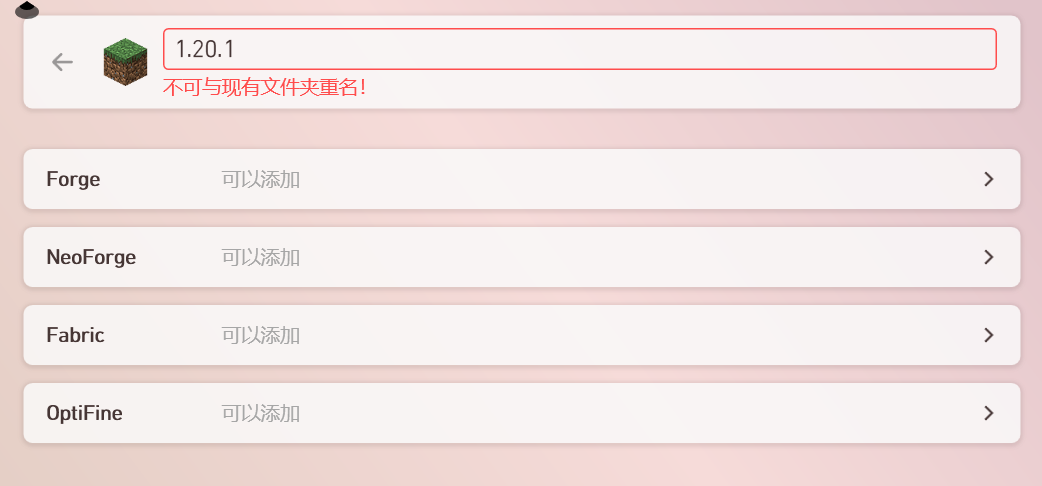
\includegraphics[width=0.7\textwidth]{./Pictures/PCL_1.jpg} %插入图片,[]中设置图片大小,{}中是图片文件名
					% \caption{Main name 2} %最终文档中希望显示的图片标题
				\end{figure}
				\par 可以看到下载页面有一堆东西,如果你要安装模组、整合包或者光影的话,请移步\hyperlink{modsinstall}{1.5 模组的安装}和\hyperlink{guangying}{1.7 光影、材质}这两章节进行阅读。
				\par 不安装,只玩原版的话,就可以点击下载了。
				\par 同时,强烈建议开启 设置→启动→默认版本隔离→隔离所有版本。不开启的话你的模组、存档等等会变得一团糟!
				\par 而在安装好java后,需要设置 设置→启动→游戏Java→自动选择合适的Java 。这样Java环境才算真正配置好。
				\par 接下来就可以启动游戏了。
				\begin{flushright}(13247903)\end{flushright}
		\subsection{正版?盗版?}
			\hypertarget{zhengbandaoban}{}
			\par 我的世界正版盗版之间的关系与其他游戏不同,在第三方启动器中下载的游戏和在官网下载的游戏其实没有任何的区别,正版盗版的唯一区别就是正版登录,也就是说我的世界的正版实际上是指正版账号,而没有正版账号的玩家可以使用离线登录(当然,这个方式在官方启动器中显然不可行,而在第三方启动器中被广泛使用)。
			\par 正版登录与离线登录似乎都能正常游玩Minecraft,但是实际上有相当大的区别,尤其是在联机服务器方面。
			\par 在正版登录下,Minecraft游戏内每个人的名称实际上是独一无二的,不允许重名的出现,因为服务器内每个人的信息,包括血量、背包内容、经验值、皮肤等等是按照游戏名储存和读取的。
			\par 但是在离线登录下,虽然个人信息依旧根据游戏名存储和读取,但是离线登录他妈压根都称不上“登录”,你在离线登陆的时候,只需要胡几把给自己取个名字,然后就能启动游戏开玩了。那我问你,输入密码的环节在哪?要是有人跟你输入了同样的名字,那他自然就相当于使用着你胡乱编出来的名字游玩,就自然拥有着你的一切。。。懂了吧?或者你第一天使用的名字是123,第二天换成321,那你在第二天进入服务器的时候,你就别再惊讶于你那空空如也的背包了。。。
			\par 虽然有些专供离线玩家游玩的服务器会选择安装登陆插件,使得玩家可以给自己的名字在进入服务器的时候注册并添加密码,但是目前学校的服务器没有添加,因为有开启正版验证的计划。
			\par 什么是正版验证?正版验证是我的世界服务器的一个登录验证选项,对于开设Minecraft服务器的人来说,可以选择在服务器配置页面开启正版验证,这样的话只有拥有Minecraft正版账号,并以正版登录方式启动游戏的人才能进入服务器。
			\par 关于网易版,网易版确实在法律层面上是正版,但似乎有人拆解网易启动器时发现其实使用的是离线登录,而网易版玩家实际上并不具有购买了我的世界的微软账户......有种广东以色列理工学院的学生实际上并没有以色列理工学院的学生账号的幽默感。
			\par 尽管考虑到购买正版需要花费89 RMB的“巨款”,我们仍然强烈建议,甚至严肃要求您购入正版,尽管目前服务器并没有开启正版验证(即目前允许离线登录玩家进入服务器)。原因如下:
			\begin{itemize}
				\item[-] 日后因为各种原因(防止不明事理的人恶意破坏服务器内设施,利用离线登录顶替他人上线,离线登录与假人模组冲突的可能性等等),服务器很有可能开启正版验证。
				\item[-] 群内有可能会有去开启了正版验证的大型服务器游玩的活动,如果你没有,你猜猜谁不会邀请?
				\item[-] 你可能已经玩了这个游戏多年了,为什么不买一个正版呢?
				\item[-] 你也不想被大家怀疑成是一个就算拿这钱去充原神月卡或者什么其他二游也不愿意购买正版 \\ Minecraft的人吧?
				\item[-] 付不起89元的人已经被上海东方明珠化身防御塔发射激光打死了,被广东以色列理工学院吉祥物蚂蚁分尸了。
			\end{itemize}
			\begin{flushright}(13247903)\end{flushright}
		\subsection{模组的安装}
			\hypertarget{modsinstall}{}
			\par 模组指的是在原版游戏之外新添加的内容,可以是辅助你玩游戏的小地图,或者是一些新内容(工业,暮色,新武器等等)。
			\par 显然,模组不是原版游戏,自然也不算是Mojang的官方内容,自然原版游戏当然不能直接运行模组文件。我们需要模组加载器。
			\par 目前主流模组加载器有:
			\par Forge:最大,最早,最全,最强,最牛逼,最屌的模组加载器,近乎支持所有的版本(从我的世界测试版/远古版到1.20.1),强强强!
			\par Neoforge:呃,1.20.1版本以及以上的forge叫这个名,因为在开发1.20.1以上版本forge时forge团队爆发了分歧,直接黑化分裂成为neoforge和forge两个团队,春日影这块。。。forge团队的原班人马目前基本都在neoforge团队,所以你可以认为forge只是在1.20.1后改了个名字,仍然强强强!
			\par Fabric:后起之秀,优化据说是比forge好(似乎,我不道啊),跟forge差不多,只是版本支持没那么好(1.14以上),强强强!
			\par 注意,forge和fabric是不可兼容的!
			\par 并且有相当一部分模组只出了这两种加载器中的一个版本,意味着另外一个版本的模组加载器压根不能运行这个模组,也就是你玩不了!
			\par 不过多数主流模组还是会提供两个加载器的版本的,不必过于惊慌。
			\par 模组也有对应的版本,你必须安装与你所游玩的游戏版本一致的模组,否则无法运行(显然,不行就是不行)。
			\par 模组加载器的下载在下载游戏中选择即可,下载后就已经包含了模组加载器。(PCL)
			\begin{figure}[H] %H为当前位置,!htb为忽略美学标准,htbp为浮动图形
				\centering %图片居中
				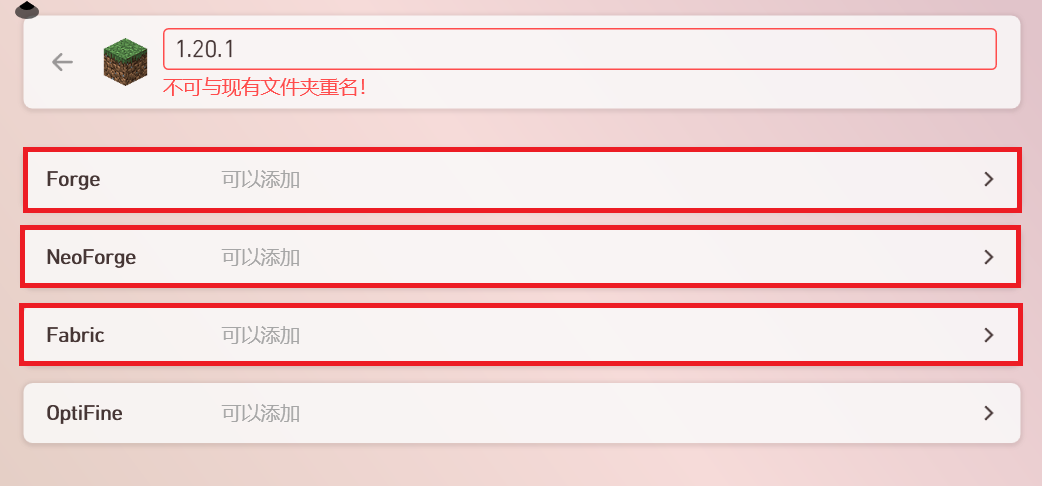
\includegraphics[width=0.7\textwidth]{./Pictures/PCL_2.jpg} %插入图片,[]中设置图片大小,{}中是图片文件名
				% \caption{Main name 2} %最终文档中希望显示的图片标题
			\end{figure}
			\par 一般选择最新版或稳定版。
			\par 模组也可以在PCL内下载,或者前往MC百科下载,不作过多阐述。
			\begin{flushright}(13247903)\end{flushright}
		\subsection{整合包的安装}
			\par 整合包,就是一堆模组打成一个包,这样就不用麻烦的一个一个下模组,只需要安装整合包即可。
			\par 各个整合包的安装方法不大一样,目前没有特别统一的方法,但是基本上是导入安装。
			\par 以生电服模组整合包为例,在群里下载下来以后,只需要将其拖到PCL页面,就可以自动导入,并且自动下载对应的版本游戏本体,所以就无需再次安装游戏,安装完成后就可以直接游玩。
			\par 其他的整合包有可能有例外,具体可以尝试找到该整合包的官方发布网站,看看如何安装,或者去MC百科查询。
			\begin{flushright}(13247903)\end{flushright}
			\par 有关我服整合包的安装,请移步\hyperlink{qidongqixuanze}{4.3 启动器选择和整合包的安装}查看。
			\begin{flushright}(9DA62C42)\end{flushright}
		\subsection{光影、材质}
			\hypertarget{guangying}{}
			\par 你觉得我的世界的光照太假了?你需要光影!
			\par 光影和模组一样,需要光影加载器,光影会重构我的世界游戏内的光照逻辑,给你更真实的游戏体验,就是可能对显卡有需求
			\par 怎么安装?自己查,毕竟这不是玩游戏必须
			\par 材质可以改变游戏内方块的样貌,给你的游戏增添不同的风格。
			\par 怎么安装?自己查,毕竟这不是玩游戏必须的
			\begin{flushright}(13247903)\end{flushright}
	\section{生电服务器}
		\subsection{什么是生电服务器?}
			\par 生电,Survival Circuit,即生存电路,通常指在原版游戏中利用游戏特性制作的红石机器。而生电服务器,就是以大量制造这类机器为特点的服务器。
			\par 制造这些机器的目的基本是用来大批量获取某些物品、方块,并且此类机器的产量十分巨大,一般会按组/小时(几组每小时)为单位计算产量,产量较高的机器甚至可以达到每小时万组甚至百万组的量级。而如此巨大的产量将会用于建造大型建筑,建造产量更大的机器等。同时这样巨量的物品也会对玩家的库存容量、物品分类等等提出挑战,需要设计专门的机器来进行分类和储存。而产量高的机器通常又需要建造空置域,这又需要玩家掏空几百个区块。。。
			\par 如果你对生电服务器仍然还是没有什么概念,你可以去b站搜索一些生电服务器视频来了解,国内比较出名的生电服务器有Tis服务器和B站up主脏小豆的服务器。而相关的UP主有火弦月、黑山大叔等等。
			\begin{flushright}(13247903)\end{flushright}
		\subsection{生电服务器的常用模组}
			\par 上文说过,生电是指存在于原版游戏中的东西,为什么这里又提到要安装模组?
			\par 这是因为原版我的世界所提供给我们的功能实在是太弱小了,没有力量!当你在专心搞建筑的时候,是不是希望自己能够按照脑中的想法快速的放置方块?是不是想方便的查看某个方块的光照强度?是不是想在修机器的时候不用拆开机器就能知道内部哪里出了问题?
			\par 不用担心!下列模组将会给你提供这些强力的功能!
			\par 投影模组:可以给你预先建造好的建筑生成一个投影文件,或者你可以在网上下载别人的投影文件,然后将文件导入游戏,就可以在服务器中显示这个建筑的投影,你接下来的工作就是照着投影一层一层逐步放置方块就行,这对大型建筑的建造十分有用!关于本mod的教程可以去b站搜索,上面已经有一万个视频讲这个了。。。
			\par minihud:一个视觉辅助类模组,可以允许你在游戏中生成一些视觉类的辅助,比如确定各个生物群系的详细边界,各个结构的具体范围,区块的加载等等。这些信息会极大的帮助刷怪塔类型的建造。b站已经有一万个视频讲如何使用这个模组了。。。
			\par Tweakeroo:如果上面两个只是视觉类的辅助,那么这个所提供的帮助就近乎于开挂了,灵魂出窍、锁定下蹲、左右键连点等等。不过,在一个非PVP类型的服务器中,你要这些功能又能有什么用呢?灵魂出窍可以让你在不破坏那些复杂机器的情况下看到机器的内部结构,锁定下蹲可以让你更加快速的建造建筑,左右键连点又可以帮你快速完成很多重复性的动作。类似的功能有很多,一万个视频在b站讲这个模组怎么使用。。。
			\par 上面是生电三大模组了可以说是
			\par 然后还有一些:
			\par 地毯模组:这个模组只需要在服务器安装,我的意思是作为玩家,你不用安装这个模组,进入服务器后仍然可以在服务器中使用这个模组(因为我们服务器已经装了)。这个模组允许玩家生成一些“假玩家”,或者通常被称之为假人。你或许已经看到过服务器里经常有名为“sand1”、“sand2”的玩家,其实那些就是假人,假人通常被用来执行一下目前生电机器仍然无法做到的事情,比如放置一个方块,破坏一个方块等等,因为Minecraft目前还没有任何机器可以做到这一点,这些东西只有玩家才能做到,所以我们可以生成一个假人,控制假人来完成某些任务。同时,假人也被广泛地被用于保持区块的加载(如果你不懂什么是区块加载,你得自己去查)。仍然有很多视频在b站上教你如何使用这个模组。
			\begin{flushright}(13247903)\end{flushright}
		\subsection{为什么?}
			\par 为什么?什么为什么?
			\par 为什么要玩生电服务器?这么做有何意义?
			\par 生电服务器可以说是一个上限很高,下限也很低的服务器了。如果你真的没有玩过或很少玩我的世界,生电服务器相比于其他服务器仍然是一个更好的选择,没有眼花缭乱的非原版模组内容,没有声嘶力竭的PVP战斗,生电服务器就是一个纯粹的原版服务器,只不过更专业,更硬核。新玩家可以在这里逐渐学习关于原版游戏的一切,而对于已经游玩了几年游戏老玩家,能容纳他们的也只有生电服务器了。
			\par 生电服务器的意义是什么,实话说谁也不知道,但是你确实是在创造着什么,可能是属于你自己的,可能是服务器玩家总体的。如果你感觉你现在只不过是为了父母而学习,为了生活而忙碌,或许你可以打开游戏为你自己创造点什么。
			\par 如果就连玩生电服务器都没有什么意义,那也就没有什么游戏有意义了。
			\begin{flushright}(13247903)\end{flushright}
	\section{本校服务器}
		\subsection{本校有什么服务器?}
			\par 截至2025.7.27,群内服务器如下:
			\par
			\par 校园生电服务器
			\par 玩了将近半年,目前服主是SharpOwO,服务器运行在服主寝室里的电脑上。
			\par IP在群公告
			\par 
			\par GTNH服务器
			\par 大型科技硬核整合包服务器,目前运行不到一个月,运行在租雇的云端服务器上(这个整合包对电脑要求太高开不起),费用需要玩家平摊。
			\par 想要进服可以联系13247903、qwqmr、蜉蝣、andarsar、Lzui37
			\par 
			\par 友情服:
			\par 茶茶小游戏服务器
			\par 我的世界小游戏服务器,有很多经典的游戏,由隔壁汕大oolong$\underline{\makebox[1ex]{}}$ttea同学开设,属于社会服务器,玩家基本为校外各路人士,所以注意信息甄别。
			\par 进服可以联系oolong$\underline{\makebox[1ex]{}}$ttea或者sharpOwO
			\par
			\par 拟建服务器:
			\par 生电创造服:
			\par 用于对生电服务器的大型建筑进行提前规划、建设、预览,创造模式,在服务器里建造的建筑会被在生电服中实装,此外该服务器不会也不应当有其他用途。
			\begin{flushright}(13247903)\end{flushright}
		\subsection{如何加入服务器?}
			\par 见\hyperlink{howtologinin}{9DA62C42编写的教程}
			\par 补充如下:
			\par 在校园中游玩服务器,强烈建议使用网线连接网络。淘宝4块就能买到一米长的,将电脑接入寝室网口,会有浏览器弹出认证窗口,只需要输入学生账号密码后认证即可使用有线连接连接服务器,使用有线连接的玩家请使用非内网穿透的IP连接服务器
			\par 有线连接的好处是可以做到0延迟,十分稳定,但是只有在学校寝室等有网线插口的地方使用,并且女生寝室D1竟然并不支持有线连接!
			\par (是认为我们女玩家不会使用有线网络吗,哈基蚁你赢了......)
			\par 所以人在D1楼层的玩家以及不在校内的无法使用有线连接的玩家,可以选择使用内网穿透连接,只需要使用内网穿透IP连接,无需网线,但是内网穿透无法承受过多的人数。
			\par 所以强烈建议有能力使用有线连接就要使用有线连接!避免挤占内网穿透的带宽!
			\begin{flushright}(13247903)\end{flushright}
		\subsection{生电服务器玩家习惯法}
			\par 之所以被称之为习惯法,就是约定俗成的法律,彼此默认的规矩,服务器的新玩家越来越多,这里也有一些提醒给新玩家。
			\par 这个服务器是生电服,生电服就是生电服,在生存模式下的服务器。
			\par 别再问为什么不能开创造了,别再问为什么不给你创造权限了,你击靶谁啊,没上完小学可以去旁边广以附校上。
			\par 目前有服务器管理权限的只有sharpOwO服主本人和13247903,服务器权限仅用于维护服务器运行,例如存档,回档等。
			\par 同时,虽然teakeroo模组所提供的功能在很多人眼中已经可以被视作作弊,在其生电服务器中被广泛认可使用,其功能确实无可替代,也确实属于辅助类型模组。但teakeroo已经是服务器规则的底线,不可以添加比tweakroo更加过分的模组,比如使用透视材质包等等,或者在2b2t无政府服务器内被广泛使用的作弊包,被发现了包给你ban了。少装懂哥,少显摆你在互联网上看过的已经烂大街的知识,一两次还能忍忍,逼装多了大伙就要讨厌你了。
			\par 生电服务器是一个工程量很大的服务器,可能每个机器动辄就需要用几十个小时才能搭建好,大型建筑则更是可能需要上万个方块,更别说空置域则需要掏空几十个区块。如此巨大的工程必然不可能由某个玩家独立完成,从建筑的构思、设计、到建造机器、生产建筑材料、实装建筑,每一步都需要许多玩家协同分工,否则则不可能完成这一壮举。所以,毫不夸张的说,服务器中几乎所有机器生产出来的资源都是每个建造这个机器的玩家的成果,所以在损坏或怀疑自己损坏了某个机器的时候,请立即在群里通知大家,方便维修或回档。
			\par 同时,生电服务器不同于其他商业性质的服务器,例如各种小游戏服务器,hypixel、网易版上形形色色的服务器,什么建筑工业拔刀剑纯净生存等等。生电服务器更像是一个邀请制的服务器,所有的成员彼此之间都熟识,这样才有条件,有能力完成分工与挑战。所以,如果你刚刚进服不知道干什么,可以在游戏里或者群里问一问目前还有哪些任务,哪些项目需要人手,可以的话可以要求给你派任务的人上线给你做指导,一般来说如果有条件的话,那个人应该会上线给你指导的,应该吧,大概也许会(
			\par 服务器的资源都是大家创造的,那么这些资源自然也属于所有人,除了一些特殊声明的用于某个工程的箱子,或者写上某个玩家ID的箱子,其他的箱子内的物资都是可以取用的。服务器的资源目前来看是产量大于消耗量的,毕竟机器的效率很高,所以不要再说类似于“嘿嘿这个箱子里的铁全是我的了,我偷偷全部拿走自己玩去了”这种话,进了服务器和大家一起玩就行了,把在商业服务器养出来的毛病改一改,大伙都是同学,有什么不可以好好交流的?再说了,服务器那刷帖机每小时能出约100组的铁锭,你拿个几盒不成问题,再这么说话,小心末地水晶变身防御塔炸你。
			\par 同时,这个生电服也是一个校园服务器,服务器成员几乎只有校内的同学,对于刚开始玩这类服务器的同学来说,请对其他成员保持尊重,虚心求教,少当那什么装逼哥,不懂装懂,对别人的成果嗤之以鼻,如果你惹了谁生气的话,请自求多福吧,可能过一会儿他就到你寝室门口了。
			\par 服务器成员时常会有线下活动,一般是出去吃饭,请关注群聊,想去都可以去。
			\begin{flushright}(13247903)\end{flushright}

	\section{如何进入我服}
		\hypertarget{howtologinin}{}
		\subsection{Java的安装}
			\subsubsection{如何选择Java版本}
				\par 在Java官网得到的安装包版本最高只有8,如需JDK24,JDK21,需要移步oracle→产品→Java并选择你需要的Java版本。
				\par 如果你需要使用本服务器的生电整合包,推荐Java17。
				\begin{flushright}(9DA62C42)\end{flushright}
			\subsubsection{对于LauncherX启动器}
				\par 如果你要使用生电整合包,那么不建议使用LauncherX启动器。
				\par 使用LauncherX启动器可以大大简化Java安装难度。打开软件→设置→Java虚拟机设定→下载 \\ Java→选择合适的版本。
				\begin{flushright}(9DA62C42)\end{flushright}
		\subsection{我服基本信息}
			\subsubsection{版本等基本信息}
				\par 版本:1.20.1,模式:纯净生存。
				\begin{flushright}(9DA62C42)\end{flushright}
			\subsubsection{连接方式}
				\par 使用网线连接校园网后在游戏内添加服务器[Github上隐藏ip],或者直接使用连接[Github上隐藏ip]。前者只有在学校内使用校园网才行。
				\par ip地址请移步我服QQ群群公告中查看。
				\begin{flushright}(9DA62C42)\end{flushright}
		\subsection{启动器选择和整合包的安装}
			\hypertarget{qidongqixuanze}{}
			\subsubsection{不建议使用的启动器}
				\par 不建议使用官方启动器,LauncherX启动器,因为无法安装整合包,如果无需模组辅助可以考虑(不建议)。
				\par 推荐使用PCL2和HMCL,如何下载请参阅\hyperlink{qidongqi}{1.3.2 启动器:启动minecraft的程序}。
				\begin{flushright}(9DA62C42)\end{flushright}
			\subsubsection{整合包在哪里?}
				\par 整合包在群文件里,搜索1.20.1,下载“1.20.1生电整合包.zip”,并且记录下载位置,之后有用。
				\begin{flushright}(9DA62C42)\end{flushright}
			\subsubsection{HMCL}
				\par 把下载的HMCL主体放在硬盘某个空白文件夹中,双击运行。
				\par 如何安装整合包:打开软件→左侧选择“版本列表”→安装整合包→导入本地整合包文件→找到整合包文件并安装。
				\begin{flushright}(9DA62C42)\end{flushright}
			\subsubsection{PCL2}
				\par 把下载的PCL2主体放在硬盘某个空白文件夹中,双击运行。
				\par 如何安装整合包:打开软件→下载→整合包→安装已有整合包→找到整合包文件并安装。
				\begin{flushright}(9DA62C42)\end{flushright}
	\section{服务器内部基本介绍}
		\subsection{末地工业区}
			\subsubsection{大致地理位置}
				\par $(100,\sim,0)$: 刷沙机(末地部分)
				\par $(326,\sim,0)$: 小黑塔
				\par $(119,\sim,-236)$: 树场
				\par $(377,\sim,-241)$: 苔藓骨粉机
				\par $(-146,\sim,-250)$: 刷石机
				\par $(-428,\sim,-423)$: 320熔炉组
				\par $(-189,\sim,-387)$: 农场
				\par $(19,\sim,-412)$: 村民交易所
				\par $(-24,\sim,-566)$: 刷铁机
				\par $(-36,\sim,-757)$: 袭击塔
				\begin{flushright}(9DA62C42)\end{flushright}
			\subsubsection{刷沙机(末地部分)}
				\par 注意:刷沙机不可空跑,运行时需要保证假人Sand1, Sand2都在线。
				\par 末地部分的刷沙机主要用于收集及固化混凝土粉末,固化功能需要手动开启。
				\par 重力方块,如铁砧、沙子、混凝土粉末在收集区域的西侧。固化后的混凝土在收集区域的东侧。
				\par 如何启用固化机:在确认刷沙机(主世界部分)只刷混凝土粉末时,在末地部分关闭坐标为 \\ (100,52,2)的拉杆,固化机会自动固化混凝土粉末并收集。
				\par 如何关闭固化机:在末地部分打开坐标为(100,52,2)的拉杆即可。
				\begin{flushright}(9DA62C42)\end{flushright}
	\section{常见问题}
		\subsection{整合包相关}
			\subsubsection{屏幕上会显示背包内容}
				\par 此现象是物品栏HUD+导致,按"I"可以关闭。此模组的按键绑定可以在选项→按键控制→按键绑定→Inventory HUD+中修改。
				\begin{flushright}(9DA62C42)\end{flushright}
			\subsubsection{飞行有问题}
				\par 如果发现鞘翅飞行有些奇怪,是因为Do a Barrel Roll模组,在启动器中关闭模组或者删除即可。
				\begin{flushright}(9DA62C42)\end{flushright}
    	\section{跋(其实就是后记,为了装逼我写跋这么个古代用词)}
			\par 如果你已经看完了本篇文章,说明你已经初步具备了一些知识,接下来打开游戏开冲!
			\par 记得把群推广给更多对我的世界感兴趣的同学,尤其是女同学,群里现在男女比例已经是地狱了,在这样下去群里就要变成美国监狱浴室了(悲)
			\begin{flushright}(13247903)\end{flushright}
\end{document}
